\clearpage
\section{Technische Grundlagen Zigbee}\label{sec:TechnischeGrundlagenZigbee}

\subsection{Netzaufbau und Topologie}\label{subsec:NetzaufbauundTopologie}
\todo[inline]{Welchen Aufbau? Welche Art von Mesh? Welche Nodetypen gibt es? Welche typischen Eigenschaften besitzt das Protokoll?}


Zigbee ist nicht gleich Zigbee. Obwohl Zigbee von zentraler Stelle, der Zigbee Alliance, spezifiziert wurde gibt es verschiedene Arten davon. In den Spezifikationen wird zwischen zwei sogenannten Stackprofilen \textit{ZigBee} und \textit{ZigBee PRO} unterschieden.
Während \textit{ZigBee}-Netzwerke eine Baumstruktur haben und der Koordinator dabei einen Single-Point-of-Failure bildet, bieten \textit{ZigBee PRO}-Netzwerke geroutete Mesh Funktionalitäten mit Routing Tabellen und Wegentdeckung. Der Koordinator bildet dabei keinen Single-Point-of-Failure mehr da sich das Routing dynamisch anpassen kann.
Die Abbildung \ref{fig:NetzwerktopologienZigbee} zeigt die Unterschiede von einem Baumnetzwerk im Stackprofil \textit{ZigBee} links und einem Meshnetzwerk im Stackprofil \textit{ZigBee PRO} rechts.
In der vorliegenden Arbeit wurde das \textit{ZigBee PRO} Stackprofil verwendet womit vollwertige Meshnetzwerke möglich sind.

\begin{figure}[h]
	\centering
	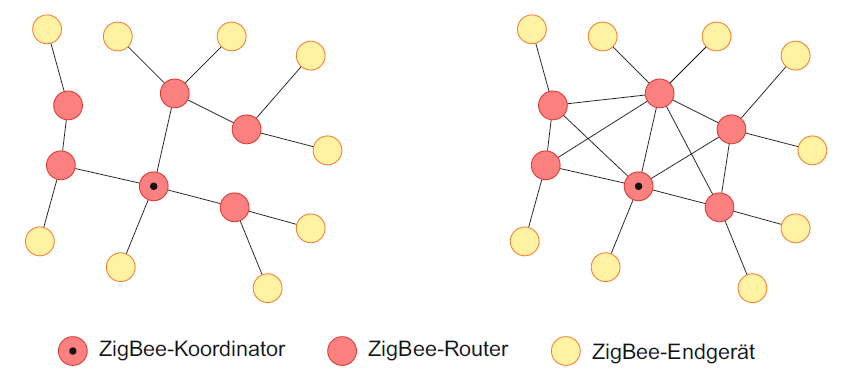
\includegraphics[width=0.8\textwidth]{Zigbee_Netztopologie.png}
	\caption{Zigbee Baum- und Meshnetzwerke in den unterschiedlichen Stackprofilen. \cite{markus_krause_rainer_konrad_drahtlose_2014}}
	\label{fig:NetzwerktopologienZigbee}
\end{figure}

Wie in der Abbildung \ref{fig:NetzwerktopologienZigbee} bereits angedeutet, kann innerhalb eines Zigbee Meshnetzwerkes zwischen 3 Nodetypen unterschieden werden. Diese besitzen unterschiedliche Aufgaben und Eigenschaften.

\paragraph{Zigbee Koordinator}\label{par:ZigbeeKoordinator}
Als zentrale Einheit übernimmt der \textit{Zigbee Koordinator} Aufgaben wie den Start und die Verwaltung eines PAN (Personal Area Network) inkl. der Definition der wichtigsten Parameter wie der PAN-ID, der Sicherheitsschlüssel sowie die Wahl des IEEE Channels.
In einem Zigbee-Netzwerk gibt es genau ein Gerät das die Rolle des \textit{Zigbee Koordinators} übernimmt. Wenn dieses Gerät das Netzwerk verlässt oder kurzzeitig ausser Betrieb ist, kann das Netzwerk trotzdem weiter bestehen und funktioniert normal weiter.
Jeder \textit{Zigbee-Koordinator} hat gleichzeitig auch die Rolle eines \textit{Zigbee-Router}.

\paragraph{Zigbee Router}\label{par:ZigbeeRouter}
\textit{Zigbee-Router} bilden das eigentliche Meshnetzwerk. Sie übernehmen die Aufgabe des Routings was die Wegentdeckung sowie Weiterleitung von Paketen beinhaltet. Jeder \textit{Zigbee-Router} führt eine Routing-Table welche fortlaufend aktualisiert wird.

\paragraph{Zigbee End-Device}\label{par:ZigbeeEndDevice}
Die einfachste Rolle ist jene des \textit{Zigbee End-Devices}. Sie stehen in einer Parent-Child Beziehung mit einem \textit{Zigbee-Router}.
Diese Kommunikation findet entweder periodisch oder ausgelöst durch einen Userinput statt.
Ankommende Pakete werden jeweils vom Parent-Node gespeichert bis das  \textit{Zigbee End-Devices} diese abruft.
\textit{Zigbee End-Devices} besitzen ausserdem keine Routing Funktionen und gelten deshalb als sehr energiesparend.
Ausgeführt als Sleepy-End-Device können CPU und RAM des entsprechenden Nodes ganz oder teilweise heruntergefahren werden und durch periodische Interrupts geweckt werden.
Dadurch können sehr lange Batteriestandzeiten erreicht werden. \cite{markus_krause_rainer_konrad_drahtlose_2014}





\subsection{Zigbee Protokoll Stack}\label{subsec:ZigbeeProtokollStack}
\todo[inline]{Erläuterung des Protokoll Stacks. Möglichst viel Grafiken und nur so viel als nötig Prosa.}



\begin{figure}[h]
	\centering
	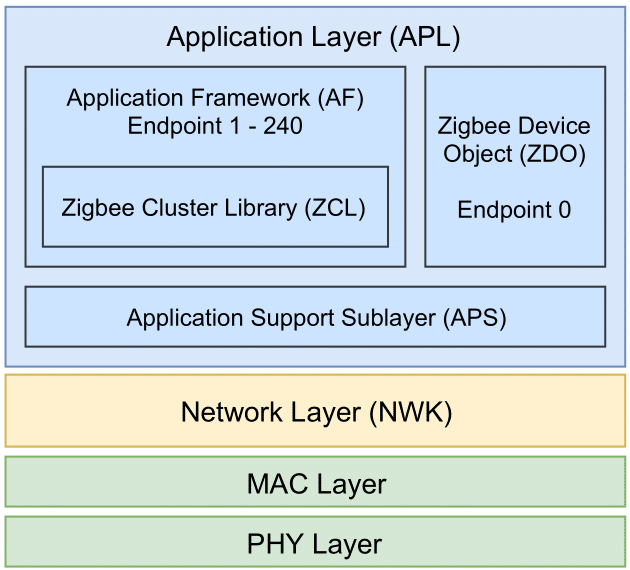
\includegraphics[width=\textwidth]{Zigbee_Architektur.png}
	\caption{Architektur des Zigbee Protokoll Stacks \cite{markus_krause_rainer_konrad_drahtlose_2014}}
	\label{fig:ArchitekturdesZigbeeProtokollStacks}
\end{figure}

\subsubsection{MAC und PHY Layer}\label{subsubsec:MACundPHYLayer}

\subsubsection{Network Layer}\label{subsubsec:Network Layer}

\paragraph{Routing}\label{par:Zigbee Routing}
\todo[inline]{Route discovery packets.}
\todo[inline]{Routing table}






\subsubsection{Application Support Sublayer (APS)}\label{subsubsec:ApplicationSupportSublayer}


\subsubsection{Application Layer}\label{subsubsec:ZigbeeApplicationLayer}

\paragraph{Zigbee Cluster Library (ZCL)}\label{par:ZigbeeClusterLibrary}

\paragraph{Endpunkte}\label{par:ZigbeeEndpunkte}





\subsection{Zigbee Software Development Kit}\label{subsec:ZigbeeSoftwareDevelopmentKit}
\todo[inline]{Eingesetzte SDK und deren Aufbau beschreiben. Allenfalls die wichtigsten API Funktionen genauer erläutern.}
